\chapter{Tinjauan Pustaka dan Dasar Teori}
Bab ini akan membahas tinjauan pustaka yang mencakup penelitian-penelitian sebelumnya sebagai referensi untuk melaksanakan tugas akhir. Selain itu, akan dijelaskan tentang teori-teori yang menjadi dasar dalam pembuatan aplikasi tugas akhir.
\section{Tinjauan Pustaka}
% ================================= Penelitian Designing Gamification for Programming Learning Applications =================================
Gamifikasi telah terbukti menjadi strategi yang efektif dalam meningkatkan minat dan motivasi belajar. 
Berdasarkan beberapa studi yang ada, pengimplementasian gamifikasi yang tepat akan meningkatkan ketertarikan dan motivasi murid dalam proses pembelajaran \cite{EnjoyLearningLikeGaming}.
Salah satu studi yang dilakukan pada tahun 2022 oleh Evan Pradanika, Yani Widyani, dan Yanti Rusmawati dengan judul \textit{Designing Gamification for Programming Learning Applications } \cite{GamificationInProgLang} membahas mengenai penerapan gamifikasi
dalam sebuah pembelajaran pemrograman. Studi tersebut menerangkan sebuah perancangan desain sistem menggunakan pendekatan \textit{Activity-centered Design} dimana perancangan ini berfokus pada aktivitas utama pembelajaran\cite{GamificationInProgLang}. 
Implementasi gamifikasi pada penelitian ini berpedoman pada hubungan antara jenis-jenis pengetahuan atau \textit{Type of Knowledge} yang memiliki elemen gamifiaksinya masing masing.
Hubungan ini dijelaskan dalam buku yang ditulis oleh Karl M. Kapp yang berjudul \textit{"The Gamification of Learning and Instruction : Game-based method and strategies for training and education"}\cite{kapp2012gamification}.
Proses pengembangan desain gamifikasi dalam penelitian ini didasari dengan kategori pembelajarannya sendiri yaitu ilmu pemrograman yang dikategorikan sebagai \textit{declarative knowledge}.
Dengan mengevaluasi aplikasi pembelajaran pemrograman yang sudah ada di pasaran, Evan Pradanika dan teman-temannya merumuskan desain tersebut berdasarkan kebutuhan user, dan aktivitas pemrogramannya sendiri.
Sehingga, elemeng gamifikasi yang digunakan dalam penelitian ini adalah
\textit{Trivia} yang diterapkan dalam latihan-latihan dalam bentuk jawaban singkat dan pilihan ganda,
\textit{Matching} diterapkan dalam latihan-latihan dalam bentuk seret dan lepas,
\textit{Challenges} diterapkan dalam bentuk prestasi yang dapat diperoleh oleh pengguna.
Keluaran dari penelitian ini ialah sebuah \textit{High-fidelity prototype} (gambar \ref*{fig:High-fidelity prototype Evan}) dari aplikasi pembelajaran pemrograman yang sudah dirumuskan.
Kemudian desain tersebut diujikan dan dievaluasi menggunakan \textit{Usability Testing dan User Experience Goals} untuk mengukur perfroma interaktif produk terhadap penggunanya.
Usability teting yang dilakukan berupa \textit{Completion Rate} untuk mengukur efektivitas, \textit{System Usability Scale (SUS)} untuk mengukur kebergunaan,
\textit{Single Ease Question (SEQ)} untuk mengukur tingkat kesulitan dari aktivitas yang diberikan, \textit{Intrinsic Motivation Inventory (IMI)} yang merupakan instrumentasi untuk mengukur motivasi,
dan \textit{User Engagement Scale-Short Form (UES-SF)} untuk mengukur keterlibatan.
% Untuk konteks pembelajaran pemrograman, pemrograman senriri dapat dikategorikan sebagai pengetahuan deklaratif karena memungkinkan pembuatan variabel dengan tipe yang telah ditentukan oleh bahasa pemrograman. 
% Selain itu, pemrograman juga termasuk ke dalam pengetahuan prosedural karena melibatkan urutan eksekusi instruksi dalam sebuah program. 
% Selanjutnya, pemrograman juga termasuk pengetahuan konseptual karena memiliki beberapa konstruksi yang dapat digunakan, seperti if-then-else dan loop, yang merupakan konsep asli dari bahasa pemrograman itu sendiri.
% \newpage
%  \begin{table}[H]
% 	\caption{Domain Pembelajaran dan Teknik Pembelajaran dan Gamifikasi Terkait \cite{kapp2012gamification}}
% 	\vspace{0.5em}
% 	\centering
% 	\begin{tabular}{|m{5cm}|m{5cm}|m{4cm}|}
% 		\hline
%         \multicolumn{1}{|c|}{\textbf{Type of Knowledge}} & \multicolumn{1}{c|}{\textbf{Gamification Elements}} & \multicolumn{1}{c|}{\textbf{Examples}} \\ 
% 		\hline 
%         \hline
% 		Declarative Knowledge & Stories/Narrative, Sorting, Matching, Replayability & Trivia, Hangman, Drag and Drop \\\hline
% 		Conceptual Knowledge & Matching and sorting, Experiencing the concept  & Wack a Mole, You Bet! \\\hline
% 		Rules-Based Knowledge  & Experience Consequences  & Board games, Simulated work tasks \\ \hline
%         Procedural Knowledge  & Software challenges, Practice & Data Miner, Software scenarios \\\hline
%         Soft Skills & Social Simulator  & Leadership simulation  \\\hline
%         Affective Knowledge & Immersion, Providing success, Encouragement from a celebrity-type figures  & Darfur Is Dying  \\\hline
%         Psychomotor Domain & Demonstration, Haptic devices  & Virtual Surgery Simulator  \\
%         \hline
% 	\end{tabular}
% 	\label{Tab: Tabel Type of Knowledge and Gamification}
% \end{table}
\newpage
\begin{figure}[htbp]
	\centering
	\begin{subfigure}[b]{0.35\textwidth}
		\centering
	  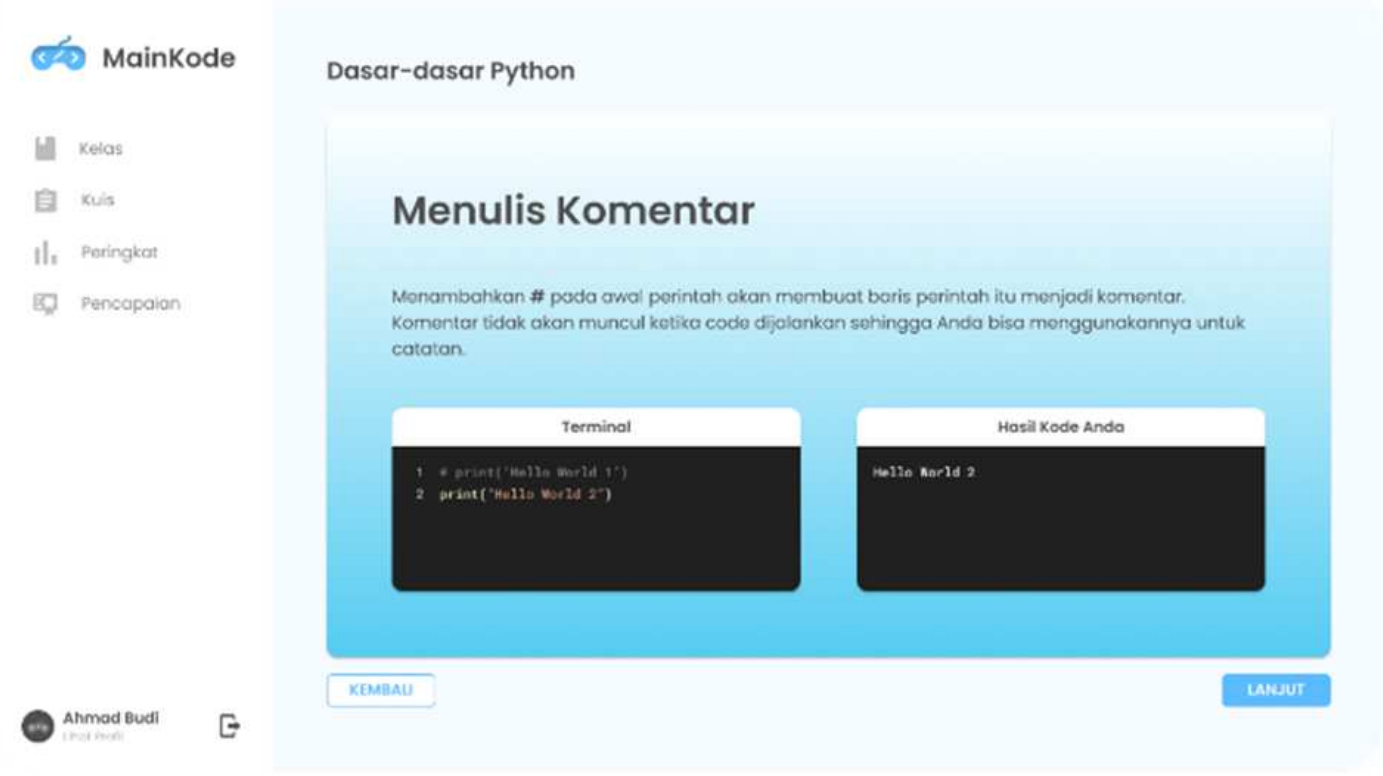
\includegraphics[width=\linewidth]{contents/chapter-2/images/Evan-a1.png}
	  \caption{\textit{Class topic page}}
	  \label{fig:sub1-a1}
	\end{subfigure}
	\begin{subfigure}[b]{0.35\textwidth}
	\centering
	  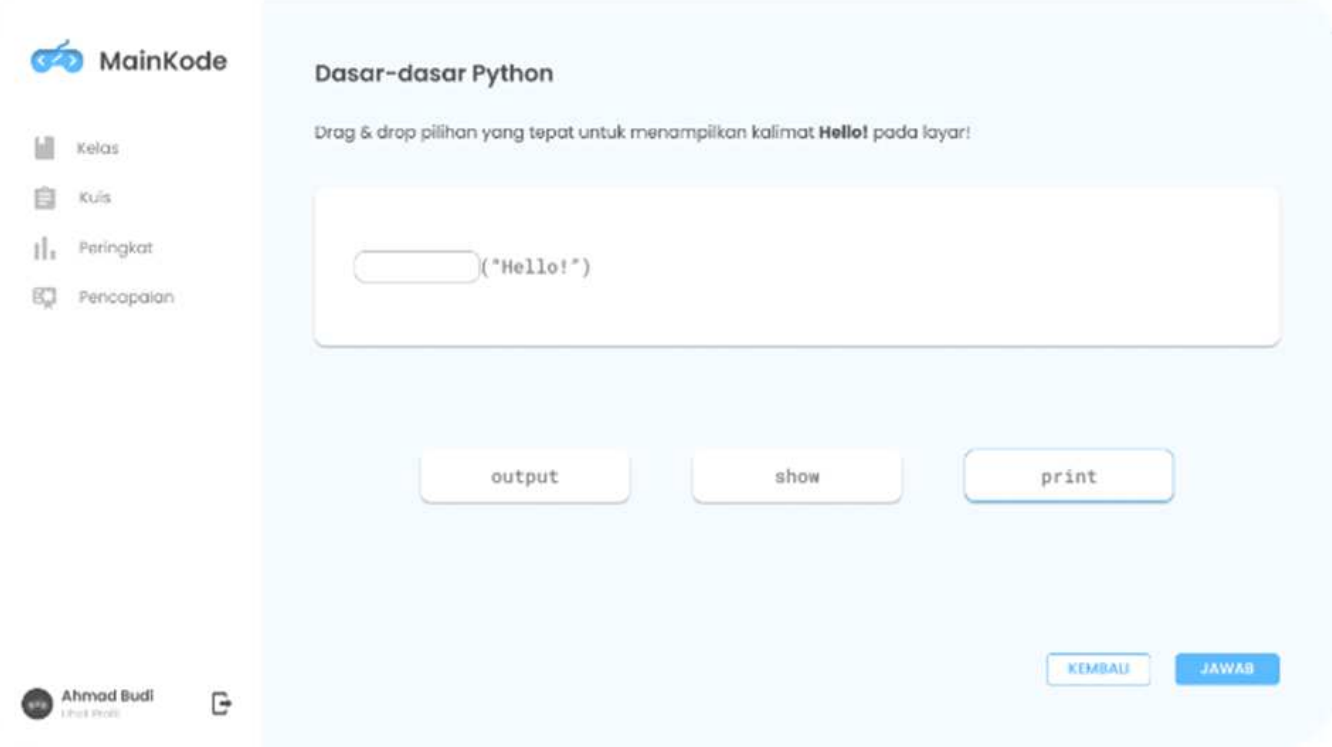
\includegraphics[width=\linewidth]{contents/chapter-2/images/Evan-a2.png}
	  \caption{\textit{Gamified exercise page}}
	  \label{fig:sub2-a2}
	\end{subfigure}
	\hfill
	\begin{subfigure}[b]{0.35\textwidth}
		\centering
		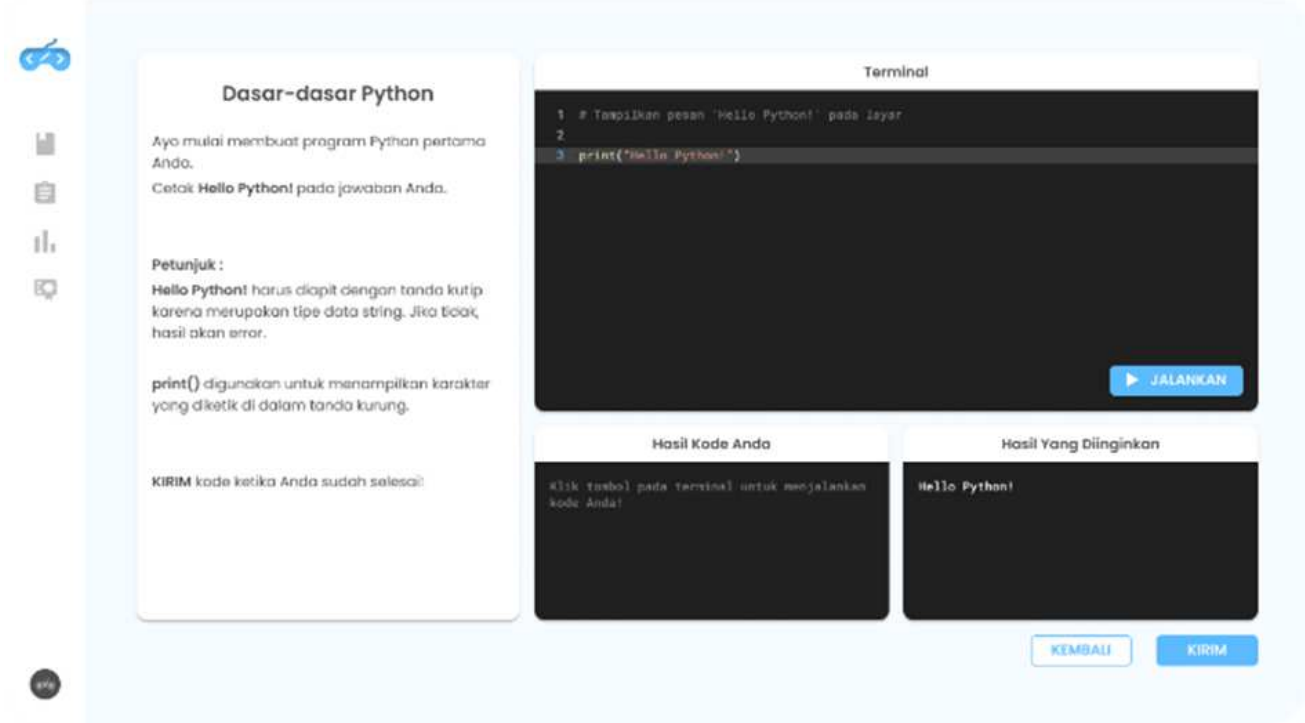
\includegraphics[width=\linewidth]{contents/chapter-2/images/Evan-a3.png}
		\caption{\textit{Terminal exercise page}}
		\label{fig:sub3-a3}
	\end{subfigure}  
	\begin{subfigure}[b]{0.35\textwidth}
		\centering
		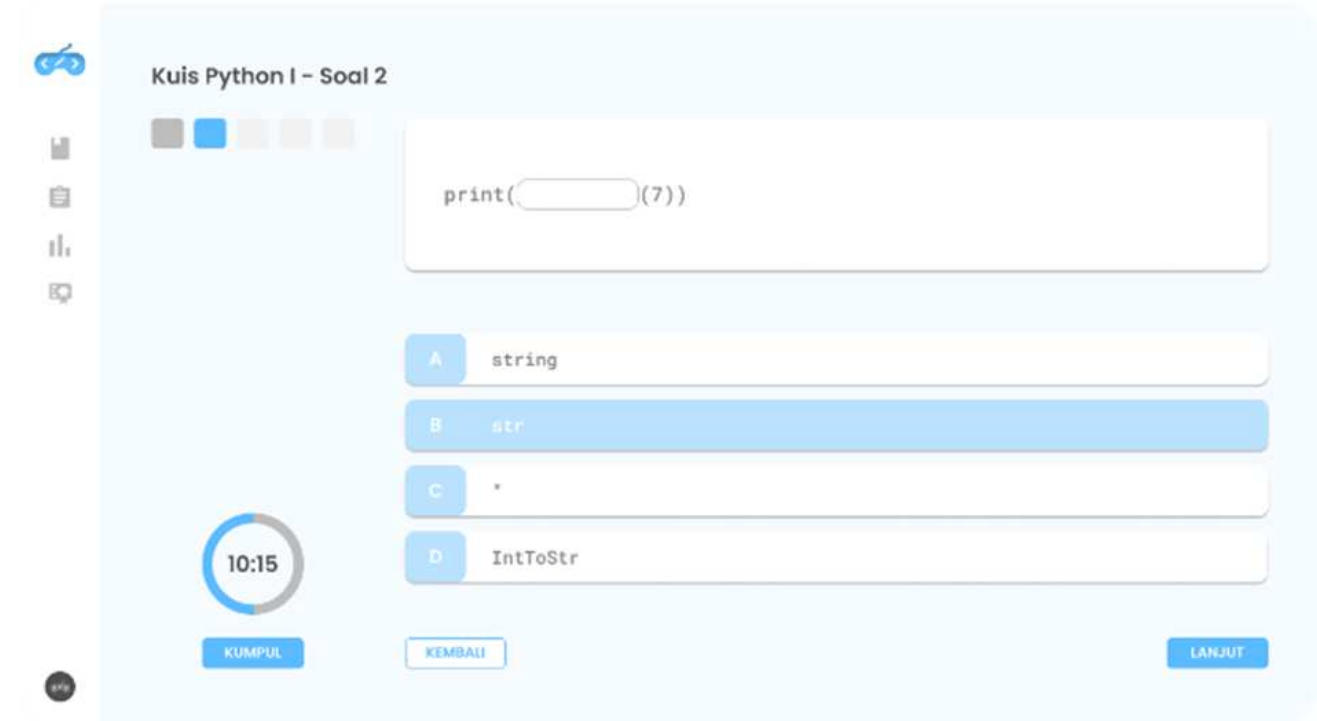
\includegraphics[width=\linewidth]{contents/chapter-2/images/Evan-a4.png}
		\caption{\textit{Quiz page}}
		\label{fig:sub4-a4}
	\end{subfigure} 
	\begin{subfigure}[b]{0.35\textwidth}
		\centering
		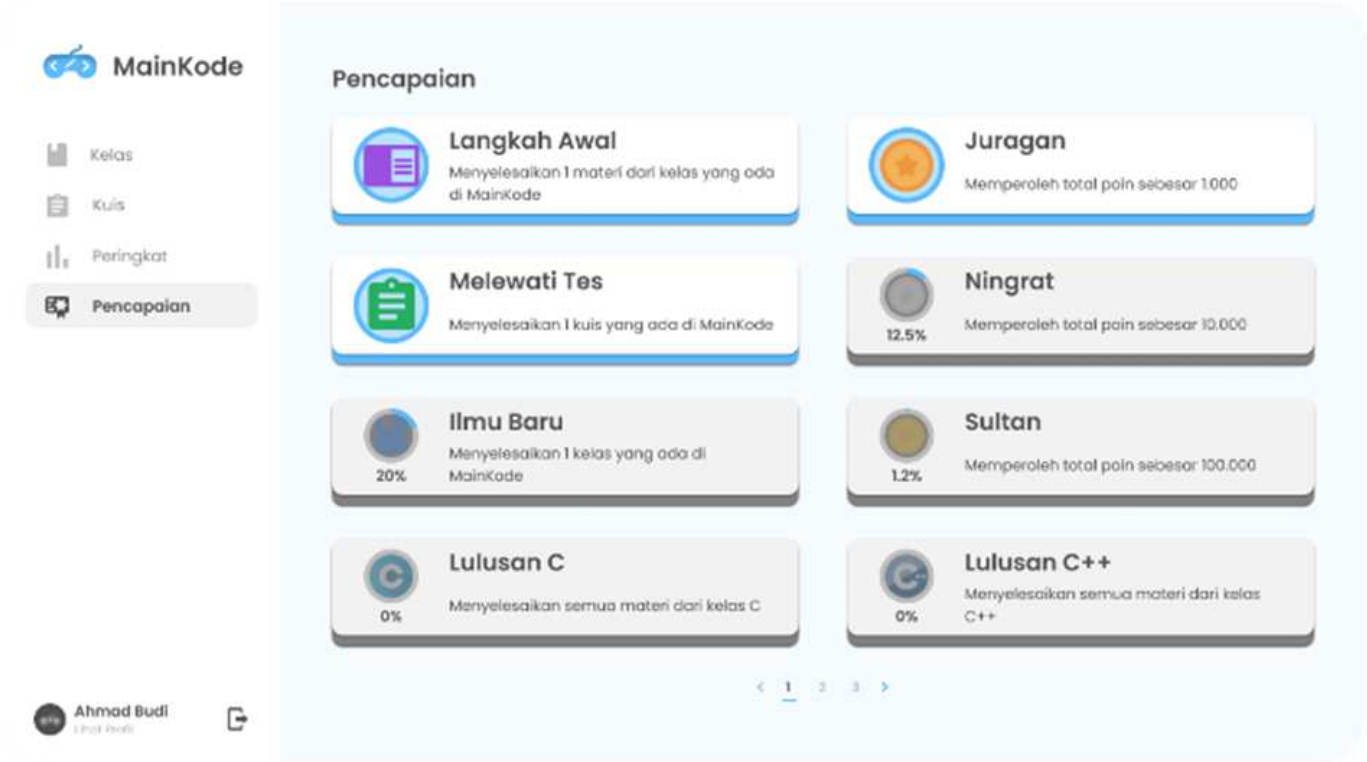
\includegraphics[width=\linewidth]{contents/chapter-2/images/Evan-a5.png}
		\caption{\textit{Achievement page}}
		\label{fig:sub5-a5}
	\end{subfigure} 
	\caption{\textit{High-fidelity prototype} aplikasi pembelajaran pemrograman}
	\label{fig:High-fidelity prototype Evan}
  \end{figure}
% ================================= Penelitian Design of Gamification for Anatomy Learning Media =================================
  Ada pula penelitian yang dilakukan pada tahun 2022 oleh 
% Metode tersebut dapat divisualisasikan dengan gambar \ref*{Fig:itterative-Design Cycle}
% \begin{figure}[H]
% 	\centering
% 	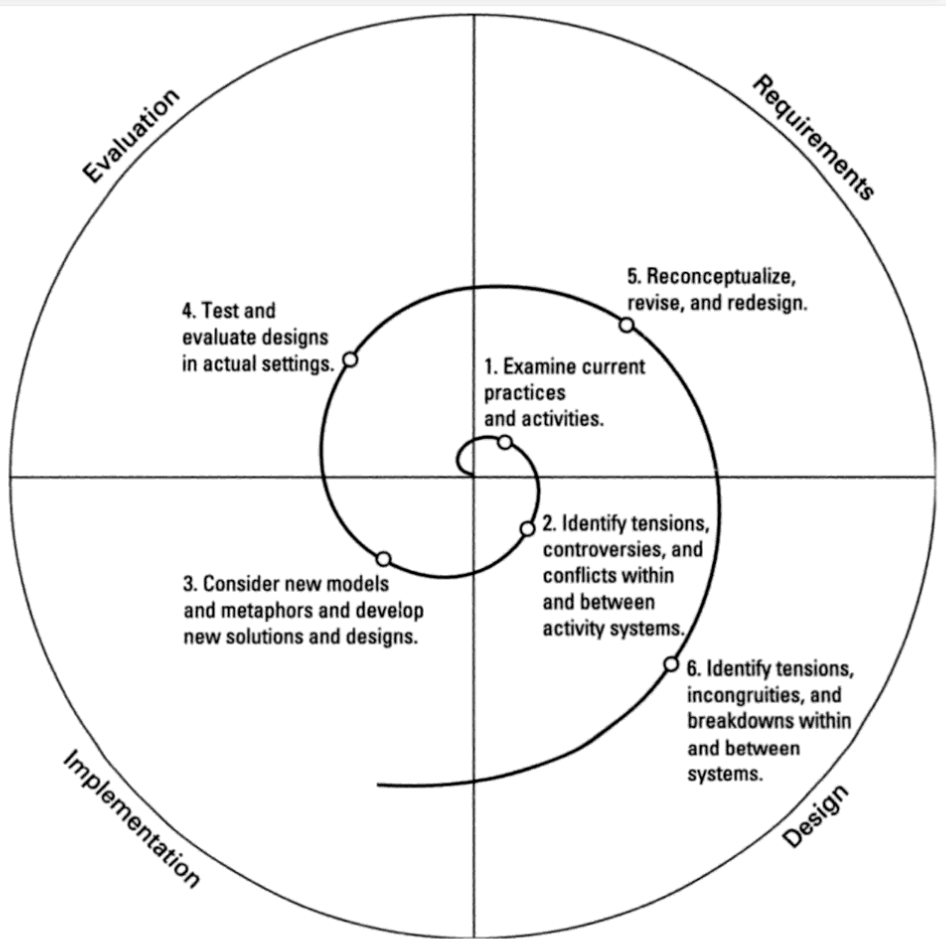
\includegraphics[width=6cm]{contents/chapter-2/images/Itterative-design.png}
% 	\caption[Caption]{An itterative-Design Cycle \cite{2004activity}}
% 	\label{Fig:itterative-Design Cycle}
% \end{figure}
\section{Analisis Perbandingan Metode}
\section{Dasar Teori}
\subsection{Media Pembelajaran}
\subsection{Teori Game}
\subsubsection{Elemental Tetrad} 
Elemental Tetrad adalah sebuah kerangka konseptual yang digunakan dalam desain dan analisis produk atau layanan digital. 
Konsep ini pertama kali diperkenalkan oleh Jesse James Garrett, seorang desainer pengalaman pengguna terkemuka, 
dan berfokus pada empat elemen utama yang saling berinteraksi dalam pengalaman pengguna digital.

\subsubsection{The MDA Framework}
MDA (Mechanics, Dynamics, Aesthetics) Framework adalah sebuah kerangka kerja yang digunakan dalam pengembangan permainan
(game development) untuk menganalisis dan memahami elemen-elemen inti yang membentuk pengalaman bermain game. 
Konsep ini pertama kali diperkenalkan oleh Robin Hunicke, Marc LeBlanc, dan Robert Zubek pada tahun 2004.
\subsubsection{The Game Design Spiral}
Game Design Spiral (lingkaran desain permainan) adalah pendekatan iteratif 
dalam desain permainan yang menggabungkan siklus pengembangan dan pengujian berulang untuk menciptakan 
permainan yang lebih baik seiring berjalannya waktu. Pendekatan ini memungkinkan desainer permainan untuk 
memperbaiki dan meningkatkan desain mereka melalui siklus yang terus berulang.
\subsection{Gamifikasi}
\subsection{FDD}
\subsection{Black Box Testing}
\subsection{\textit{System Usability Testing}(SUS)}
\subsection{\textit{User Experience Questionnaire}(UEQ)}


% Di dalam tinjauan pustaka hasil akhirnya adalah analisis secara kualitatif atau pun secara kuantitatif kelebihan dan kekurangan metode jika dikaitkan dengan masalah, batasan-batasan masalah dan solusi yang dinginkan.
% Analisis kuantitatif tidak wajib teapi mempunyai nilai tambah di dalam tugas akhir saudara. Bagian ini menjelaskan kenapa metode tersebut dipilih dan uraikan dengan lebih jelas metode pelaksanaan tugas akhir yang ingin Anda lakukan. 
% \section{Pertanyaan Tugas Akhir (Jika Perlu)}

% Pertanyaan tugas akhir bersifat opsional dan dapat ditambahkan untuk menekankan hal-hal yang hendak diketahui dari tugas akhir berdasar pada tujuan tugas akhir. Pertanyaan tugas akhir dikenal dengan RQ (\textit{Research Question}) dan harus memiliki keterkaitan dengan RO (\textit{Research Objective}). Satu RO dapat memiliki satu atau lebih dari satu RQ. 

